\section{Performance + Portability}


Until now, I looked at performance and portability separately which is OK since sometimes one is only interested in one of these aspects. 
One may know that the code will only ever be executed on one specific hardware platform, and it is important to achieve the best performance possible down to the assembly level. 
On the other hand, for some, it may be enough to write code that can be executed everywhere but that must not necessarily be performant. 
However, for many achieving a combination of both is also important: writing code that can be executed on a variety of different hardware, without the need to re-implement everything from scratch again if the hardware changes, but that also achieves reasonable performance on all hardware. 
By reasonable here I mean that it achieves a high enough fraction of the possible achievable performance. 
It should be clear that it is extremely difficult or even impossible to achieve the same performance with code that can run on all \glspl{gpu} and \glspl{cpu} there are compared to highly optimized vendor-specific solutions that may even be implemented by the vendors themselves with special closed-source knowledge of the underlying hardware. 

Assessing performance portability is an ongoing research topic. 
Over the years, many definitions emerged starting with more informal definitions of performance portability. 
Note that the following definitions aren't exhaustive but only serve as examples.


%%% QUOTES - informal Performance Portability definitions


In 2013 in their original Kokkos paper \citeauthor{edwards_kokkos_2013} defined performance portability as:
\begin{quotebox}{\citet{edwards_kokkos_2013}}
    Our performance portability objective is to maximize the amount of user code that can be compiled for diverse devices and obtain the same (or nearly the same) performance as a variant of the code that is written specifically for that device.
\end{quotebox}
While this definition was already quite good, the problem is that \enquote{\textit{nearly the same}} can and will be interpreted differently by different people. 
Therefore, this definition is not feasible to use as an object performance portability metric.

In 2014 \citeauthor{kunkel_performance_2014} defined performance portability as:
\begin{quotebox}{\citet{kunkel_performance_2014}}
    A code is performance portable if it can achieve a similar fraction of peak hardware performance on a range of different target architectures.
\end{quotebox}
As with the quote from \citeauthor{edwards_kokkos_2013} the problem is the objectivity of the definition namely how big the \enquote{\textit{similar fraction of}} should be. 
Although \citeauthor{kunkel_performance_2014} stated that for them it is \SI{20}{\percent} of the \enquote{best achievable performance} with respect to a hand-optimized native implementation, another person could argue that it should be \SI{15}{\percent} or \SI{25}{\percent} making this metric also highly subjective. 

In 2016 \citet{larkin_performance_2016} defined performance portability as:
\begin{quotebox}{\citet{larkin_performance_2016}}
    The same source code will run productively on a variety of different architectures.
\end{quotebox}
Again, \enquote{\textit{productively}} is highly subjective not only in a performance but also in a portable way. 
This definition can include that maintaining custom code paths for better performance may be ok as long as it is not too much work. 

Also in 2016, the \gls{doe} conducted a meeting \cite{neely_doe_2016} specifically regarding performance portability. 
There, a few attendees were asked to define performance portability in their own words:
\begin{quotebox}{Rob Neely~\cite{neely_doe_2016}}
    For purposes of this meeting, it is the ability to run an application with acceptable performance across KNL and GPU-based systems with a single version of source code.
\end{quotebox}
\begin{quotebox}{Simon Pennycook~\cite{neely_doe_2016}}
    An application is performance portable if it achieves a consistent level of performance (e.g. defined by execution time or other figure of merit, not percentage of peak flops across platforms relative to the best known implementation on each platform.
\end{quotebox}
\begin{quotebox}{Adrian Pope, Vitali Morozov~\cite{neely_doe_2016}}
    Hard portability = no code changes and no tuning. Software portability = simple code mods with no algorithmic changes. Non-portable = algorithmic changes.
\end{quotebox}
\begin{quotebox}{David Richards~\cite{neely_doe_2016}}
    A code is performance portable when the application team says its performance portable!
\end{quotebox}

At the end of the \gls{doe} meeting, the attendees also created a working definition trying to incorporate the above definitions into one: 
\begin{quotebox}{\gls{doe} Working Definition~\cite{doe_meeting_attendees_definition_nodate}}
    An application is performance portable if it achieves a consistent ratio of the actual time to solution to either the best-known or the theoretical best time to solution on each platform with minimal platform specific code required.
\end{quotebox} % https://performanceportability.org/perfport/definition/

As with all other previous definitions, all of these quotes contain some objective part in one way or another.
However, to discuss performance portability objectively, these subjective definitions can not be used if it is expected that everyone should agree on the same values. 


%%% formal Performance Portability definitions


Therefore, the first objective performance portability metric was introduced by \citeauthor{pennycook_implications_2019} at the end of 2016 published on arXiv~\cite{pennycook_metric_2016}, and finally submitted as a full paper at the beginning of 2017~\cite{pennycook_implications_2019}. 
It was the first formal definition that can be used to assess the performance portability of an application objectively.

\begin{definition}[Performance Portability \pp~(Pennycook et al.~\cite{pennycook_implications_2019})]\label{def:pp}
    Given a problem $\mathbf{p}$ which is solved by an application $\mathbf{a}$ and a set of platforms $\mathbf{H}$, the performance portability metric \pp is defined as:

    \[ \pp(a, p, H) = 
        \begin{cases}
            \frac{\abs{H}}{\sum\limits_{i \in H} \frac{1}{e_i(a, p)}} & \text{if }i\text{ is supported } \forall i \in H \\
            0                                                         & \text{otherwise}
        \end{cases} 
    \]

    where $\mathbf{e_i}$ is the performance efficiency of $\mathbf{a}$ solving $\mathbf{p}$ on platform $\mathbf{i \in H}$.
\end{definition}

Therefore, the performance portability metric \pp is the harmonic mean over the performance efficiency of an application solving a specific problem on all tested hardware platforms. 
The only difference to the harmonic mean is that \pp is also defined if the input data, i.e., the performance efficiency, includes a $0$. 
The \pp metric has the nice property that, per construction, it is in the interval $\interval{0}{1}$ where $0$ means the application did not run on all hardware platforms and $1$ means the best possible performance on all hardware platforms. 

Note that \pp heavily emphasizes the \textit{portability} aspect of performance portability: If only one hardware platform is not supported the result of \pp will directly be $0$ regardless of the performance on all other hardware platforms. 
Depending on your target audience, this property of \pp may be desirable or not. 

\todo{Marowka's Kritik aufzählen}
\cite{marowka_toward_2021, marowka_reformulation_2022, marowka_comparison_2023, marowka_portability_2024, marowka_inorrect_2024}

\todo{highlight \textbf{same architecture class}}

\begin{definition}[Performance Portability \mpp~(\citet{marowka_comparison_2023})]\label{def:mpp}
    Given a problem $\mathbf{p}$ which is solved by an application $\mathbf{a}$ and a set of supported platforms $\mathbf{S \subseteq H}$ from the same architecture class, the performance portability metric $\overline{\pp}$ is defined as:

    \[ \mpp(a, p, S, H) = 
        \begin{cases}
            \frac{\sum\limits_{i \in S} e_i(a, p)}{\abs{S}} & \text{if }\abs{S} > 0 \\
            0                                               & \text{otherwise}
        \end{cases} 
    \]

    where $S \coloneqq \{ i \in H | e_i(a, p) > 0 \}$ and $\mathbf{e_i}$ is the performance efficiency of $\mathbf{a}$ solving $\mathbf{p}$ on platform $\mathbf{i \in H}$.
\end{definition}

In contrast to \pp, \mpp is defined as the normal mean across all \textbf{supported} platforms. 
The value of \mpp is $0$ if and only if \textbf{no} hardware platform in $\mathbf{H}$ is supported by the current application $\mathbf{a}$. 
This also shows us the main emphasis of \mpp in contrast to \pp: For \mpp the \textit{performance} aspect of performance portability is heavily emphasized since an application that does not run on all hardware platforms is not penalized as with \pp. 

\todo{way more complex metric}
As a response to \citeauthor{marowka_comparison_2023} critic to their performance portability metric \pp, \citet{pennycook_revisiting_2021} updated their metric to include \todo{was kam dazu?}


\citet{harrell_effective_2018} extended the performance portability even further to an \textit{effective performance portability} that does not only include the above-discussed performance portability but also the productivity, i.e., the effort a programmer has to make to achieve said performance portability. 
This metric also penalizes frameworks that achieve good performance portability but only by drastically increasing the programmer's effort, e.g., introducing special code paths for some hardware platforms. 
However, in the remainder of this thesis, I will mainly focus on \textit{performance portability} only. \todo{Begründung?}


\todo{order}
%%% performance efficiency metrics


Both formal performance portability definitions---\pp and \mpp---use a \textit{performance efficiency} $\mathbf{e_i(a, p)}$ in their definition which describes the relation between the achieved performance with respect to some proven expected performance. 
In general, two different definitions defining the performance efficiency of an application $\mathbf{a}$ solving problem $\mathbf{p}$ on the hardware $\mathbf{i \in H}$ are used. 

\begin{definition}[Architectural Efficiency]\label{def:arch_eff}
    The achieved performance as a fraction of the \enquote{peak} theoretical hardware performance, being it the achieved \si{\flop\per\second} or memory bandwidth.
\end{definition}

The \textit{architectural efficiency}

\begin{definition}[Application Efficiency~(\citet{satish_can_2012})]\label{def:app_eff}
    The achieved performance as a fraction of the \enquote{best} observed performance. 
\end{definition}

The \textit{application efficiency}

\todo{3-P challenge: performance, portability, and productivity}

\subsection{Examples}

\begin{table}[]
    \centering
    \begin{tabular}{c|C{1.5cm}|C{1.5cm}|C{1.5cm}|C{1.5cm}}
        \multirow{2}{*}{Platform Set $\mathbf{H}$} & \multicolumn{2}{c|}{Application 1}     & \multicolumn{2}{c}{Application 2}     \\
                                                   & Arch. Eff.        & App. Eff.          & Arch. Eff.        & App. Eff.         \\\midrule
        A                                          & \SI{40}{\percent} & \SI{100}{\percent} & \SI{30}{\percent} & \SI{90}{\percent} \\
        B                                          & \SI{20}{\percent} & \SI{85}{\percent}  & \SI{30}{\percent} & \SI{85}{\percent} \\
        C                                          & \SI{15}{\percent} & \SI{60}{\percent}  & \SI{15}{\percent} & \SI{40}{\percent} \\
        D                                          & --                & --                 & \SI{40}{\percent} & \SI{70}{\percent}
    \end{tabular}
    \caption{%
    Example architectural (arch. eff.) and application (app. eff.) efficiencies for two example applications on four different hardware platforms. 
    Note that the application 1 does not support the architecture D. 
    }
    \label{tab:platforms_example}
\end{table}

\todo{update table}
\begin{table}[]
    % https://www.programiz.com/online-compiler/0apVuVZDNe38e
    \centering
    \begin{tabular}{c|rrrr}
        
        Application 1           & \multicolumn{2}{c}{$\pp(a, p, H)$}          & \multicolumn{2}{c}{$\mpp(a, p, S, H)$}   \\
        Subsets of $\mathbf{H}$ & Arch. Eff.           & App. Eff.            & Arch. Eff.        & App. Eff.            \\\midrule
        \{ A \}                 & \SI{40}{\percent}    & \SI{100}{\percent}   & \SI{40}{\percent} & \SI{100}{\percent}    \\
        \{ A, B \}              & \SI{26.67}{\percent} & \SI{91.89}{\percent} & \SI{30}{\percent} & \SI{92.5}{\percent}  \\
        \{ A, B, C \}           & \SI{21.18}{\percent} & \SI{78.06}{\percent} & \SI{25}{\percent} & \SI{81.67}{\percent} \\
        \{ A, B, C, D \}        & \SI{0.0}{\percent}   & \SI{0.0}{\percent}   & \SI{25}{\percent} & \SI{81.67}{\percent} 
    \end{tabular}
    \caption{%
    The calculated values for \pp and \mpp for application 1 using different subsets of $\mathbf{H}$ and the performance efficiencies given in \autoref{tab:platforms_example}. 
    This example shows the differences between \pp and \mpp if the unsupported hardware platform D is added to the platform set $\mathbf{H}$.
    }
    \label{tab:pp_app_1_example}
\end{table}

\begin{table}[]
    % https://www.programiz.com/online-compiler/0apVuVZDNe38e
    \centering
    \begin{tabular}{c|rrrr}
        Application 2           & \multicolumn{2}{c}{$\pp(a, p, H)$}          & \multicolumn{2}{c}{$\mpp(a, p, S, H)$}      \\
        Subsets of $\mathbf{H}$ & Arch. Eff.           & App. Eff.            & Arch. Eff.           & App. Eff.            \\\midrule
        \{ A \}                 & \SI{30}{\percent}    & \SI{90}{\percent}    & \SI{30}{\percent}    & \SI{90}{\percent}    \\
        \{ A, B \}              & \SI{30}{\percent}    & \SI{87.43}{\percent} & \SI{30}{\percent}    & \SI{87.5}{\percent}  \\
        \{ A, B, C \}           & \SI{25}{\percent}    & \SI{62.66}{\percent} & \SI{25}{\percent}    & \SI{71.67}{\percent} \\
        \{ A, B, C, D \}        & \SI{25.26}{\percent} & \SI{64.35}{\percent} & \SI{28.75}{\percent} & \SI{71.25}{\percent}
    \end{tabular}
    \caption{%
    The calculated values for \pp and \mpp for application 2 using different subsets of $\mathbf{H}$ and the performance efficiencies given in \autoref{tab:platforms_example}. 
    This example shows the differences between \pp and \mpp if all hardware platforms in the platform set $\mathbf{H}$ are supported.
    }
    \label{tab:pp_app_2_example}
\end{table}
\subsection{Visualization of Performance Portability}

\citet{sewall_interpreting_2020} 
different visualization strategies:
\begin{itemize}
    \item Box Plots: obscures the "did not run" case (large boxes); no number of supported platforms; only median to compare in case of "did not run" (boxes cover whole range)
    \item Histograms: distribution of bins ("did not run" must be own bin; how many bins?); areas of low density $\rightarrow$ difficult to "see" the distribution
    \item Probability Density Function: primary problem choosing a good kernel bandwidth; PP sparse and uneven distributed data $\rightarrow$ no fixed bandwidth guaranteed to yield satisfactory results $\rightarrow$ adaptive methods; problems on [0, 1] boundaries $\rightarrow$ there may be many points there for PP making this problem even worse; but better than Histograms (better tendencies; less crowded bars)
    \item Violin Plots: a combination of kernel density estimation and Box Plots

    % Impact of Platform Selection
    \item plotting \pp against $\mathcal{H}$ $\rightarrow$ other paper \cite{deakin_performance_2019}
    \item Efficiency Cascade Plots + Platform Charts: minimum efficiency and H $\rightarrow$ remove platform with minimum efficiency and start again; independent for each application; platform sets at the bottom may not be the same for each application; monotonic decreasing
\end{itemize}

\todo{Plot script anpassen und für mich unnötiges Zeug rauswerfen.}
\begin{figure}
    \centering
    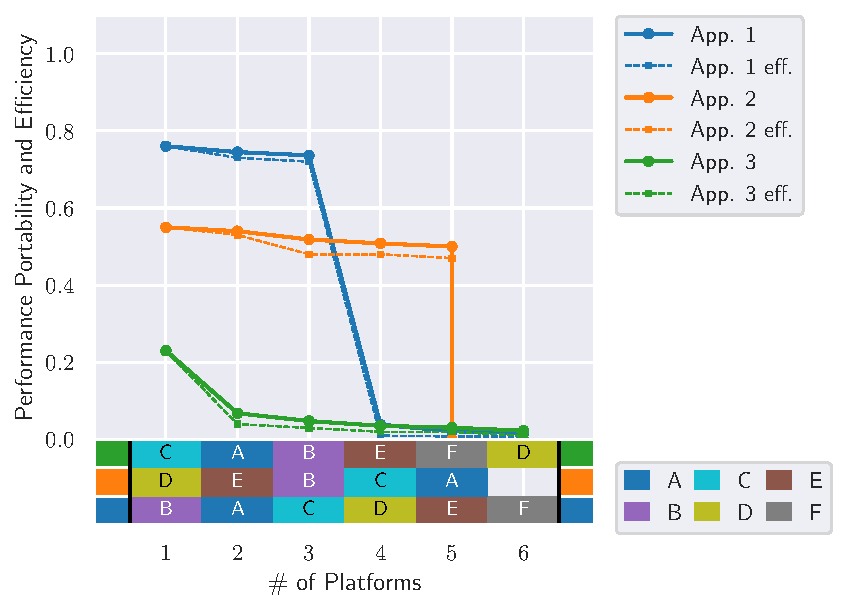
\includegraphics[width=\linewidth]{figures/02_performance_portability/example_diss_eff_cascade.pdf}
    \caption{%
    An example visualization of the performance efficiencies of \autoref{tab:platforms_example} and performance portability metrics of the two example applications from \autoref{tab:pp_app_1_example} and \autoref{tab:pp_app_2_example} as proposed by \citet{sewall_interpreting_2020}. 
    TODO: further description, falsch für \mpp?
    }
    \label{fig:pp-example-visualization}
\end{figure}

\newpage
\cite{pennycook_implications_2019}

\todo{irgendwie folgende Punkte noch unterbringen}
\begin{itemize}
    \item genaue Beschreibung von "platform": a specific hardware, OS, runtime system, etc. $\rightarrow$ hier \textbf{hardware}
    \item genaue Beschreibung von "application": software, die auf ihre Korrektheit überprüft werden kann $\rightarrow$ portability nicht nur definieren als "kann darauf laufen" sondern zusätzlich such "produziert korrektes resultat
    \item productivity schwierig zu messen/nicht objektiv, da sehr von skillset des jeweiligen Programmierers abhängig
    \item also formal Definition vor Pennycook rein?: Performance Portability on EARTH: A Case Study Across Several Parallel Architectures,
    \item arch: kann 100\% peak sein aber trotzdem nicht performant (z.B. bandwidth bound); z.B. via Roofline Model
    \item app: best known != best possible
    \item efficiency: 1 best possible; the lower, the worse
    \item 5 Kriterien an \pp aufnehmen?
    \item arch vs app : was rauslesen wenn eines klein, anderes groß
\end{itemize}

Performance Definition
\begin{quotebox}{\cite{pennycook_implications_2019}}
    Any measurable property of an application’s correct execution of a problem on a platform.
\end{quotebox}

Portability Definition
\begin{quotebox}{\cite{pennycook_implications_2019}}
    The ability of an application to execute a problem correctly on a given set of platforms.
\end{quotebox}

Performance Portability muss folgendes haben: 
\begin{itemize}
    \item beide obigen Definitionen nicht verletzen
    \item objektiv messbar, quantifizierbar und vergleichbar sein
\end{itemize}

Ihre Definition:
\begin{quotebox}{\cite{pennycook_implications_2019}}
    A measurement of an application’s performance efficiency for a given problem that can be executed correctly on all platforms in a given set.
\end{quotebox}


Current Problems in Performance Portability:
\begin{itemize}
    \item "abstraction and irreducible complexity": best Performance ohne spezialisierte Code-Pfade $\rightarrow$ hohe Abstraktionsebene, automatische Code-Generierung für performance
    \item "(still) no silver bullet": 
\end{itemize}

Approaches to Code Spezialization
\begin{itemize}
    \item libraries
    \item DSL
    \item Portability and Productivity Frameworks
    \item Autotuning
    \item Application-specific abstractions
    \item performance portable algorithms

    \item we use frameworks + autotuning in the remainder of this work
    \item for more information on vor- und nachteile see paper \cite{pennycook_implications_2019}
\end{itemize}

Criteria: (verbatim quote)
\begin{enumerate}
    \item Be measured specific to a set of platforms of interest $\mathcal{H}$.
    \item Be independent of the absolute performance across $\mathcal{H}$.
    \item Be zero if a platform in $\mathcal{H}$ is unsupported, and approach zero as the performance of platforms in $\mathcal{H}$ approaches zero. 
    \item Increase if performance increases on any platform in $\mathcal{H}$.
    \item Be directly proportional to the sum of scores across $\mathcal{H}$.
\end{enumerate}

\newpage
\cite{marowka_toward_2021}

\begin{itemize}
    \item Hauptproblem: harmonic mean
    \item Criterion 5 verletzt
    \item Criterion 3 (0 wenn cannot run) only a constrained because of the harmonic mean being undefined for $0$ values
    \item \pp to broad; research results are therefore unrealistic or biased
    \item geometric + harmonic mean won't work, arithmetic does 
    \item new platform, wobei das Verhältnis der Summe aller scores ($e_i$) gleich bleibt, ändert das Verhältnis von \pp
    \item Hat Probleme mit $0$ wenn nicht unterstützt
    \item harmonic mean tends to track more the lower values $\rightarrow$ in general smaller \pp than \mpp values
    \item calculate values for, e.g., CPUs and GPUs separately
    \item if we have no baseline (except a time that would be included in \pp), exclude it from \mpp
\end{itemize}

erste Definition:
\begin{definition}[Performance Portability \mpp~(\citet{marowka_comparison_2023})]\label{def:mpp}
    Given a problem $\mathbf{p}$ which is solved by an application $\mathbf{a}$ and a set of supported platforms $\mathbf{H}$ from \textbf{the same architecture class}, the performance portability metric $\overline{\pp}$ is defined as:

    \[ \mpp(a, p, H) = 
        \begin{cases}
            \frac{\sum\limits_{i \in H} e_i(a, p)}{\abs{H}} & \text{if }i\text{ is supported }\forall i \in H \\
            \textit{not applicable}                         & \text{otherwise}
        \end{cases} 
    \]

    where $\mathbf{e_i}$ is the performance efficiency of $\mathbf{a}$ solving $\mathbf{p}$ on platform $\mathbf{i \in H}$.
\end{definition}
$\rightarrow$ update of criterion 3 with \textit{not applicable}

\newpage
\cite{marowka_reformulation_2022}
$\rightarrow$ extended paper from \cite{marowka_toward_2021}

\begin{itemize}
    \item \enquote{Just because there is no implementation for a single architecture in |H|, for whatever reason, to conclude that the application is not at all portable and its = 0\% is unrealistic.}
    \item Observation 1: Verhältnis wird nicht gewahrt, wenn man eine platform hinzufügt
    \item Observation 2: Probleme mit application efficiency also baseline (ein $a$ nehmen, das schon in \pp mit drin ist)
    \item Observation 3: contradictions Aufgrund von 0
    \item Observation 4: problem if $0$
    \item Observation 5: Probleme, wenn man komplett unterschiedliche Architekturen anschaut (CPU vs GPU bspw.)
    \item Observation 6: do not change between baselines (may result in efficiencies greater 1 but that mahct nichts aus)
    \item \pp GENERELL abhängig von der input Größe
    \item arch vs app efficiency: bei einem bleiben!; peak vs roofling: peak schlechtere Zahlen, aber einheitlich, roofline "fairer" aber uneinheitlich; app eff: NUR wenn es eine optimierte Fassung für alle hardware gibt, nicht in \pp pder \mpp mit aufnehmen! \\$\rightarrow$ app nehmen wenn so eine baseline exisitiert, sonst arch 
\end{itemize}

Redefinition Problem: 
\begin{quotebox}
    computational problem is a collection of questions that computers might be able to solve
\end{quotebox}

application $\rightarrow$ case-study application
\begin{quotebox}
    A given case-study application is a problem that is computationally solved by an algorithm for a given set of input parameters, which is implemented in a performance portability framework, and which is mapped onto a back-end programming model and executed on a given architecture.
\end{quotebox}

Usage Guidelines (copied verbatim) $\rightarrow$ schreiben, was wir davon in späteren Kapiteln einhalten?
\begin{itemize}
    \item It is advisable not to calculate the value of \mpp for platforms of different architecture classes together, such as CPUs and GPUs. If that is what the evaluator is looking for, then it is advisable to present the scores of each architecture class separately.
    \item It is preferable to use the architectural efficiency approach instead of the application efficiency approach.
    \item It is advisable, when using the application efficiency approach, to choose the performance of a low-level, nonportable, and well-optimized implementation as the performance baseline and not to include its score in calculating \mpp.
    \item It is advisable, when using the architectural efficiency approach, to choose theoretical peak performance as the performance baseline.
    \item It is advisable not to include outlier results in calculating \mpp.
    \item It is advisable to include platforms from various vendors in the set of platforms H.
    \item It is advisable that the set of platforms H be as large as possible.
    \item It is advisable that every implementation of the case-study application use the same input parameters, implement the same algorithm, and be compiled by the same compiler and backend compiler.
\end{itemize}

% https://www.digit.in/features/apps/rainbows-unicorns-and-performance-portability-34524.html


\newpage
\cite{pennycook_revisiting_2021}

weitere Kritik: \cite{yokota_beginners_2018, bertoni_performance_2020, siklosi_heterogeneous_2018}

Criteria explained:
\begin{enumerate}
    \item results must be tied to a set of platforms in order for the results to be useful; es ist eben interessant \pp auf unterschiedlicher Hardware (CPUs und GPUs) gemeinsam zu betrachten
    \item differences in the capabilities of $H$ should not bias the results
    \item $0$ als "did not run" macht es vergleichbarer und intuitiver, das sich schlechte Performance der $0$ annähert
    \item encourage users to improve performance across all platforms of interest
    \item original goal \enquote{that comparisons of performance portability reflect comparisons of performance} $\rightarrow$ flaw lies within the criterion and \textbf{not} the formula $\rightarrow$ outliers shouldn't artificially inflate the \pp score $\rightarrow$ after tests, criterion should be discarded
\end{enumerate}

revised criteria:
\begin{enumerate}
    \item Be measured specific to a set of platforms of interest H.
    \item Be independent of the absolute performance of each platform in H.
    \item 
    \begin{enumerate}
        \item Take a numeric value for any set of platforms H.
        \item Be zero if any platform does not run; go to zero as performance on any platform in H goes to zero.
    \end{enumerate}
    \item Increase or decrease if performance increases or decreases on any platform in H, respectively.
\end{enumerate}

Advanced formula: extending \pp to all platforms in H \textbf{executing all problems in P}:

\[ \pp(a, \mathcal{P}, H) = 
        \begin{cases}
            \frac{\abs{\mathcal{P}}\times\abs{H}}{\sum\limits_{p \in \mathcal{P}}\sum\limits_{i \in H} \frac{\Lambda_{i, p}}{\lambda_{i, p}}} & \text{if }\forall i \in \abs{H}\text{ and }\forall p \in \abs{\mathcal{P}}, \lambda_{i, p} \neq 0 \\
            0                         & \text{otherwise}
        \end{cases} 
    \]

\begin{itemize}
    \item do not remove outliers $\rightarrow$ WHAT is a outlier? Maybe outliers reflect the way an application is written?
    \item hergeleitet von "first level principles" $\rightarrow$ \pp soll dadurch interpretierbarer werden
    \item \pp und \mpp: \enquote{alternative weightings of the same underlying summation} $\rightarrow$ weighting by $\frac{\Lambda_i}{\lambda_i}$  vs $\frac{\lambda_i}{\Lambda_i}$
    \item \enquote{\mpp reflects the aggregate throughput that an application would achieve when distributed across H, rather than the aggregate throughput that it should achieve.}
    \item new formula: average over averages $\rightarrow$ information for specific problem lost, but good for summarizing
    \item \enquote{Recall that \pp represents the maximum amount of work when all platforms execute for the same amount of time}
\end{itemize}



\newpage
\cite{marowka_comparison_2023}

\begin{itemize}
    \item versteht nicht, wieso einfach Criterion 5 entfernt wurde
    \item immer noch der Meinung, dass $0$ keinen Sinn ergibt
    \item $\rightarrow$ only include platforms that are supported in \mpp; "not applicable" changed to $0$ such that only numeric values are present
\end{itemize}

Revised criteria for \mpp with $S \in H$
\begin{enumerate}
    \item measured specific to a set of platforms of interest S;
    \item independent of the absolute performance across S;
    \item zero if none of the platforms is supported;
    \item increasing or decreasing if performance increases or decreases on any platform in S;
    \item directly proportional to the sum of scores across S.
\end{enumerate}

neue Formel:
\[ \mpp(a, p, H) = 
        \begin{cases}
            \frac{\sum\limits_{i \in S} e_i(a, p)}{\abs{S}} & \text{if }\abs{S} > 0 \\
            0                         & \text{otherwise}
        \end{cases} 
\]
where $S \coloneqq \{ i \in H | e_i(a, p) > 0 \}$

\begin{itemize}
    \item \pp Hauptproblem: tracks low values $\rightarrow$ architectural efficiency typically on the low side (mostly for CPUs) $\rightarrow$ \pp doesn't really track improvements
    \item proportionality one of the main goals $\rightarrow$ removed from \pp $\rightarrow$ why?
    \item not comparable
    
\end{itemize}

Problems with \cite{smith_characterizing_1988} (copied):
\begin{enumerate}
    \item Smith proved nothing. He used only one hypothetical example and deduced from it two properties that would have been desirable to include in practical and realistic benchmarks.
    \item Smith was looking at how to summarize rates (mflop/s). In contrast, the \pp metric deals with summarizing performance efficiencies that are fractions (or ratios) and are unitless.
    \item Smith emphasized in both properties that the single-number performance measure must be directly or inversely proportional to the total time.  In other words, Smith required the existence of a criterion (5) that Pennycook and Sewall chose to exclude from the criteria of the \pp metric.
    \item revised metric \pp: only applicable for arch eff and not app eff
    \item thinks outliers should be ignored in the \mpp calculation $\rightarrow$ (me:) WHY?
    \item nicht gut, dass es unterschiedliche eff $e$ gibt (erschwert reproduzierbarkeit) $\rightarrow$ arch eff via Roofline Model am wengisten reproduzierbar
\end{enumerate}


\newpage 
\cite{marowka_portability_2024}

\begin{itemize}
    \item arch eff: peak vs actual (roofline)
    \item app eff: nicht BESTE existierende Implementierung, sondern BESTE Implementierung INNERHALB der aktuellen case study (ups :D)
    \item .
\end{itemize}

\begin{quotebox}{\citet{marowka_portability_2024}}
    “the performance portability score increases or decreases if the performance increases or decreases on any platform in S.” However, the performance of OpenACC, OpenMP, and Kokkos did not increase or decrease on any platform in S ! This is clearly a contradiction
\end{quotebox}

Solutions: 
\begin{enumerate}
    \item only use arch eff if (2) and (3) are not applicable
    \item always use low-level languages as baseline (e.g., CUDA or HIP); assumption: these implementations are always the fastest
    \item Vorschlag eines "Performance Portability Repositories" wo alle optimalen application sdrin liegen sollen $\rightarrow$ immer nur die als baseline nehmen!
    \item \enquote{makes it possible to examine, based on the same data, the impact of each architecture on the performance portability of the entire application}
    \item \enquote{he portability efficiency approach explicitly defines the performance cost involved in a one-way migration of the application from a source platform to a target platform}
\end{enumerate}

\begin{definition}[Portability Efficiency~(\citet{marowka_portability_2024})]\label{def:pp_eff}
For a given base platform $\mathbf{b}$ and a target platform $t$, the portability efficiency $\eta$ of application $\mathbf{a}$ solving problem $\mathbf{p}$ on platform $\mathbf{t}$, when it is transferred from platform $\mathcal{b}$, is defined as the achieved performance of application $\mathbf{a}$ on platform $\mathbf{t}$, with the best-performing application setting on platform $\mathbf{b}$, $C(b)$, as fraction of the best observed performance of application $\mathbf{a}$ on platform $\mathbf{t}$:

\[
    \eta(a, p, b \rightarrow t) = \frac{P_{d, C(a)}}{P_{t, C(t)}}
\]
\end{definition}

\begin{definition}[Cardinality~(\citet{marowka_portability_2024})]\label{def:pp_eff_cardinality}
For a given supported set of platforms $S \clap H$ where $\abs{S} > 1$, the cardinality of s set $\mathbf{D}$ of ordered selections (permutations) of two platforms from a set of $\abs{S}$ platforms is: 

\[
    D = 2 \cdot \binom{\abs{S}}{2} = \frac{\abs{S}!}{(\abs{S} - 2)!}
\]
\end{definition}

\begin{definition}[\mpp with Portability Efficiency~(\citet{marowka_portability_2024})]\label{def:pp_eff_pp}
$$\mpp(a, p, S, H) = 
        \begin{cases}
            \frac{\sum\limits_{\{i, j\} \in D} [\eta(a, p, i \rightarrow j)]}{\abs{D}} & \text{if }\abs{S} > 1 \\
            0                         & \text{otherwise}
        \end{cases}$$

\end{definition}

\newpage
\cite{daniel_applying_2019}

$P_D$ doesn't capture performance and portability across platforms

$$P_D = \frac{\sum\limits_{i \in H} \Delta_{RMS}}{\abs{H}}$$

\begin{itemize}
    \item take problem size into account (since performance may depend on it)
    \item not a measure of productivity, but how smooth or though porting effort can be
\end{itemize}

\begin{definition}[Code Divergence~\cite{daniel_applying_2019}]\label{def:code_div}
The code divergence $\mathbf{D}$ is the average of the pairwise distances between applications in the set of codes $\mathbf{A}$:

$$D(A) = \binom{\abs{A}}{2}^{-1} \sum\limits_{\{a_i, a_j\} \subset A} d(a_i, a_j)$$

with $A \subset A_p$, where $A_p$ is the set of all applications which solve $p$. The distance $d(a_i, a_j)$ between applications $a_i$ and $a_j$ is the change in the number of LOC normalized to the smaller (in LOC) application:

$$d(a_i, a_j) = \frac{\abs{\text{LOC}(a_i) - \text{LOC}(a_j)}}{\min(\text{LOC}(a_i), \text{LOC}(a_j))}$$
    
\end{definition}

question: can I single problem accept different input data and produce different output data? $\rightarrow$ new definition of a problem:
\begin{itemize}
    \item \enquote{a problem is a proposed question that requires an algorithm to be solved correctly}
\end{itemize}

\begin{definition}[Performance Distance~\cite{daniel_applying_2019}]\label{def:perf_dist}
Given a set of applications $\mathbf{A_p}$ that solve problem $\mathbf{p}$, let $f_i(a, p, s)$ be a measure of performance of application $\mathbf{a}$ on solving $\mathbf{p}$ on platform $\mathbf{i}$ with input size $\mathbf{s}$. 
The performance distance $\mathbf{\delta(a, \alpha}$ between applications $a$ and $\alpha$ is the relative error in performance.

$$\delta(a, \alpha) = \frac{\abs{f_i(a, p, s) - f_i(\alpha, p, s}}{f_i(\alpha, p, s)}$$

Note that $f_i(\alpha, p, s)$ is the observed result or the theoretical hardware performance. 
\end{definition}

\begin{definition}[Divergence RMS~\cite{daniel_applying_2019}]\label{def:div_rms}
The Divergence RMS $\Delta_{RMS}$ is the root mean square of performance distances between a set of input sizes of interest $S$:

$$\Delta_{RMS} = \sqrt{\frac{\sum\limits_{s \in S} \delta(a, \alpha)^2}{\abs{S}}}$$

\end{definition}

\begin{definition}[Performance Portability Divergence $\mathcal{P_D}$~\cite{daniel_applying_2019}]\label{def:pp_div}
The Performance Portability Divergence $\mathcal{P_D}$ is the arithmetic mean of RMS divergences across a set of platforms $H$:

$$\mathcal{P_D} = \frac{\sum\limits_{i \in H} \Delta_{RMS}}{\abs{H}}$$

\end{definition}

\begin{itemize}
    \item optimal $\mathcal{P_D}$ would be $\SI{0}{\percent}$
    \item penalizes large performance distances severely
    \item can be larger than $\SI{100}{\percent}$
    \item easy to reach $\SI{0}{\percent}$, than $\SI{100}{\percent}$ in \pp
\end{itemize}

\newpage
\cite{sedova_high-performance_2018}

\enquote{The $PP_{MD}$ metric purports to evaluate performance portability but in practice it measures the price in performance that must be paid to make the application portable.} -- \cite{marowka_comparison_2023}

\begin{definition}[Portability \citet{sedova_high-performance_2018, mooney_bringing_1997}]
An application can be said to be portable if the cost of porting is less than the cost of re-writing:
$$DP = 1 - (\frac{C_P}{C_R}$$
where $C_P$ is the cost to port and $C_R$ the cost to rewrite the program. 
\end{definition}

\begin{itemize}
    \item $1$ $\rightarrow$ completely portable
    \item positive $\rightarrow$ porting is more profitable
    \item binary vs source code portability
\end{itemize}

\begin{definition}[MD Performance Portability~\citet{sedova_high-performance_2018}]

$$PP_{MD_c}(a, p, Q) = 
    \begin{cases}
        \frac{\abs{Q}}{\sum\limits_{i \in Q} S_i(a, p)} & \text{if }\abs{G} - \abs{Q} \neq 0\text{ and }\abs{G} - \abs{Q} \neq \abs{G} \\
        1  & \text{if }\abs{G} - \abs{Q} = \abs{G}\\
        0  & \text{if }\abs{G} - \abs{Q} = 0
    \end{cases}
$$

where $\abs{G}$ is the the cardinality of the set $G$ of algorithmic or programmatic components that significantly accelerate a best-performing application $a$, $\abs{Q}$ is the cardinality of the set $Q$ of all non-portable such accelerating components of $a$, $p$ are the parameters used in $a$, and $S$ is the speedup that this non-portable component $i$ of the application provides to the program: $S_i = \frac{T_0}{T_i}$, with $T_i$ as the time-to-solution with the use of $i$, and $T_0$ the time-to-solution without $i$.
\end{definition}

\begin{itemize}
    \item $G$: instruction-level, thread-level, process-level, or library-level
    \item $PP_{MD_c}$ not close to $\SI{100}{\percent}$: viele optimierte Teile eines Codes müssten getauscht werden mit portable Code (mit ähnlicher Performance)
    \item $PP_{MD_c}$ does not support multiple platforms
\end{itemize}

Summary of recommendations for portability (copied verbatim)
\begin{itemize}
    \item High-level programming interface with re-targetable back end that is standardized and supported by a number of both commercial and open-source initiatives.
    \item Encapsulation of machine specific sections of the program.
    \item An agreement about the worthiness of the portability effort.
    \item Modularity of the algorithm sections and the data structures, with an ability to rearrange data storage and even to change the algorithm if required.
    \item Use of only the portable subset of the standard language.
    \item A dedicated portable design effort and clear portability goals.
\end{itemize}

\newpage
\cite{bertoni_performance_2020}

\pp insufficient (same \pp values for vastly different behavior) $\rightarrow$ also use standard deviation to accomplice \pp 

\begin{itemize}
    \item roofline schwierig zu erlangen 
    \item teilweise hier schon inconsistent
    \item durch haminic mean: gleiches \pp, trotz drastisch unterschiedlichen verhalten (einmal alle ungefähr gleich; einmal in schwacher und in sehr starker run)
    \item geben zusätzlich Standardabweichung an
\end{itemize}


\newpage
\cite{yang_empirical_2018}

\begin{itemize}
    \item Roofline model as \textit{performance efficiency metric}
    \item Paper hauptsächlich wie man in "gutes" Roofline Model aufbaut
    \item 
\end{itemize}

\begin{definition}[Roofline Performance Efficiency~\citet{yang_empirical_2018}]\label{def:roof_eff}
Given the observed code performance in floating point operations per second (\si{\flop\per\second}) $P_i(a, p)$, the peak \si{\flop\per\second} $F_i$ of architecture $i$, the peak bandwidth $B_i$ of architecture $i$, and the arithmetic intensity $I_i(a, p)$ of application $a$ on architecture $i$, the Roofline performance efficiency is defined as:

$$e_i(a, p) = \frac{P_i(a, p)}{\min(F_i, B_i \times I_i(a, p))}$$
\end{definition}
The denominator accounts for when the application is compute or bandwidth bound.


\newpage
\cite{harrell_effective_2018}

\begin{itemize}
    \item not only performance portability, but productivity 
    \item critic: \pp does not penalize "heroic" optimizations efforts to increase its score (i.e., optimized code paths for specific architectures) $\rightarrow$ wouldn't be productive
\end{itemize}



\newpage
\cite{zhu_performance_2007} (before the age of GPUs)

\begin{quotebox}{\citet{zhu_performance_2007}}
    If one parallel implementation of one application already achieves good performance on one platform, can this implementation also achieve the same or similar performance on other platforms?
\end{quotebox}

\begin{definition}[Performance Portablity $P^\mathcal{P}_n(b \rightarrow t$~\citet{zhu_performance_2007}]
Given a parallel program $\mathcal{P}$ developed on the \textbf{base system}, let $S^B_n$ denote the absolute speedup achieved by $\mathcal{P}$ on $n$ computing nodes of the \textbf{base system}, and $S^T_n$ denote the absolute speedup achieved by $\mathcal{P}$ on $n$ computing nodes of the \textbf{taregt system}, then the \textbf{performance portability} on $n$ computing nodes for porting the program $\mathcal{P}$ from the \textbf{base system} to the \textbf{target system} is:

$$P^\mathcal{P}_n(b \rightarrow t) = \frac{S^T_n}{S^B_n} \times \SI{100}{\percent}$$
\end{definition}

\begin{itemize}
    \item may be greater than $\SI{100}{\percent}$
    \item \enquote{Speedup, which is a measurement of the scalability of a parallel program, also reflects the performance portability of a parallel program in the sense that performance is portable with the increase of number of processors.}
\end{itemize}



\newpage
\cite{marowka_performance_2022}

\begin{itemize}
    \item new PP metric that is not application but programming model centric
    \item again based on \mpp
    \item achieved performance of a portable programming model $M$ as a fraction of the performance of a non-portable architecture-specific parallel programming model
    \item the better, the more case studies are included
    \item again, removes outliers (ist das WIRKLICH sinnvoll?)
    
\end{itemize}

\begin{definition}[Performance Portability of a Model~\citet{marowka_performance_2022}]
The arithmetic mean of the performance efficiencies, which are the achieved performance values of a given portable model as a fraction of the performance values of a non-portable architecture-specific model, obtained from collections of case studies carried out on platforms of the same class of pairs (application, problem).
\end{definition}

\begin{definition}[Performance Portability of a Model~\citet{marowka_performance_2022}]
The performance portability metric $\mpp_M$ of a high-level portable parallel model $M$ executing a set of case studies $T$, where each $t \in T$ corresponds to application $a$ solving problem $b$  on platform $c$ is: 

$$\mpp_m = \frac{\sum\limits_{i \in T} e_(a, b, c)}{\abs{T}}$$

where $e_i(a, b, c$ is the performance efficiency of application $a$ solving problem $p$ on platform $c$.
\end{definition}



\newpage
\cite{pennycook_navigating_2021}

\begin{itemize}
    \item it should be clear what is part of the application and what of the platform (e.g., third-party libraries)
    \item Cascade plots: \enquote{applications extending further to the right support more platforms (portability), and if they do so with higher efficiency, are more performance portable.}
    \item Productivity: subjective, approximation sufficient; they use \cite{harrell_effective_2018} code divergence with the Jaccard distance
    \item dendrogram for visualizing code divergence (by clustering)
    \item \pp-CC charts: $2D$-plane, top-right corner is the goal
    \item track performance portability and productivity yas early as possible in the development process
    \begin{enumerate}
        \item identify the destination
        \item get your bearings
        \item chart the course
        \item set sail
    \end{enumerate}
\end{itemize}

\begin{definition}[Jaccard Distance SLOC~\citet{pennycook_navigating_2021}]
Given $c_i(a, p)$ as the set of source lines required to compile application $a$ and execute problem $p$ for platform $i$, the dissimilarity of the source code can be expressed as:

$$d_{i, j}(a, p) = 1 - \frac{\abs{c_i(a, p) \cap c_j(a, p)}}{\abs{c_i(a, p) \cup c_j(a, p)}}$$
\end{definition}
Here, $0$ means \enquote{single-source}, i.e., everything is shared by both platforms, and $1$ means nothing is shared. 

\begin{definition}[\pp-CC Metric~\citet{pennycook_navigating_2021}]
    $$M(a, p, H) = \min(\pp(a, p, H), CC(a, p, H))$$
\end{definition}

\newpage
\cite{yokota_beginners_2018}

\begin{itemize}
    \item tension between performance improvement and performance portability improvement
    \item \enquote{we empirically analyze the usability and usefulness of PPM, applied for OpenACC applications}
    \begin{enumerate}
        \item calculating PPM for multiple applications and platforms
        \item interpreting the results from the perspective of performance portability across devices
        \item attempting to improve the performance portability, i.e., increase PPM
    \end{enumerate}
    \item arch eff: compute-bound $\rightarrow$ operational throughput; memory-bound $\rightarrow$ bandwidth
    \item Problem arch eff: does not show whether the implementation \textbf{is actual efficient} (e.g., unnecessary memory loads, floptimization)
    \item same problem as in other studies: \pp heavily penalizes even one small performance efficiency value
    \item also points out the problem with different architecture (CPUs vs GPUs)
    \item low \pp: low efficiencies overall or big differences among platform-specific performance efficiencies
    \item how to improve low \pp?: add more platforms, use fewer platforms, improve performance efficiency
    \item \pp should be extended to include some kind of heterogeneity score
    \item trying to improve the performance efficiency $\rightarrow$ tension
    \begin{enumerate}
        \item performance \enquote{increases on all platforms}
        \item performance \enquote{increases on one platform, but decreases on another platform}
    \end{enumerate}
    \item did optimize the OpenACC code but it seems that not the baseline CUDA code $\rightarrow$ does the app eff still make sense?
    \item 
\end{itemize}

\begin{definition}[Architectural Efficiency~\citet{yokota_beginners_2018}]
    $$e\_arch_i(a, p) = 
    \begin{cases}
        \frac{OpT^{app}}{OpT^{HW}} & \text{if } OI^{app} \geq OI^{HW} \\
        \frac{BW^{app}}{BW^{HW}} & \text{otherwise}
    \end{cases}$$
    
\end{definition}

\newpage
\cite{hoefler_scientific_2015}

\begin{itemize}
    \item experimental design (for reproducibility): application, input, compiler, runtime environment, machine, and measurement methodology
    \item interpretability: \enquote{We call an experiment interpretable if it provides enough information to allow scientists to understand the experiment, draw own conclusions, assess their certainty, and possibly generalize results}
\end{itemize}

Rules:
\begin{enumerate}
    \item When publishing parallel speedup, report if the base case is a single parallel process or best serial execution, as well as the absolute execution performance of the base case.
    \item Specify the reason for only reporting subsets of standard benchmarks or applications or not using all system resources.
    \item Use the arithmetic mean only for summarizing costs. Use the harmonic mean for summarizing rates.
    \item Avoid summarizing ratios; summarize the costs or rates that the ratios base on instead. Only if these are not available use the geometric mean for summarizing ratios.
    \item Report if the measurement values are deterministic. For nondeterministic data, report confidence intervals of the measurement.
    \item Do not assume normality of collected data (e.g., based on the number of samples) without diagnostic checking.
    \item Compare nondeterministic data in a statistically sound way, e.g., using non-overlapping confidence intervals or ANOVA.
    \item Carefully investigate if measures of central tendency such as mean or median are useful to report. Some problems, such as worst-case latency, may require other percentiles.
    \item Document all varying factors and their levels as well as the complete experimental setup (e.g., software, hardware, techniques) to facilitate reproducibility and provide interpretability.
    \item For parallel time measurements, report all measurement, (optional) synchronization, and summarization techniques.
    \item If possible, show upper performance bounds to facilitate interpretability of the measured results.
    \item Plot as much information as needed to interpret the experimental results. Only connect measurements by lines if they indicate trends and the interpolation is valid.
\end{enumerate}

Additional: 
\begin{itemize}
    \item report units unambiguously
    \item costs: metrics with a direct semantic (runtime, energy consumption, number of instructions)
    \item rates: derived from costs (\enquote{if the denominator has the primary semantic meaning, the harmonic mean provides correct results})
    \item ratios (unitless): should never be averaged
    \item statistical methods instead of arithmetic ones (samples must be normal distributed and either costs or rates): 
    \begin{itemize}
        \item standard variation
        \item coefficient of variation (good for performance consistency of a system over longer time)
        \item confidence interval of the mean
    \end{itemize}
    \item median and quartiles
    \item confidence intervals of the median
    \item recommend not to remove outliers
    \item analysis of variance (ANOVA)
    \item quantile regression
    \item factorial design
    \item warm-up, warm vs cold cache
    \item power-of-two best case for some algorithms (e.g., MPI\_Reduce)
    \item string vs weak scaling
    \item full benchmarks vs kernel benchmarks
    \item measure single events
    \item in general more than $5$ runs
    \item three cases of bounds models:
    \begin{itemize}
        \item ideal linear speedup
        \item serial overheads (Amdahls's law)
        \item parallel overheads
    \end{itemize}
    \item Points should only be connected if they indicate a trend and values between two points are expected to follow the line
\end{itemize}

% https://intel.github.io/p3-analysis-library/